\documentclass[conference]{IEEEtran}
\IEEEoverridecommandlockouts
% The preceding line is only needed to identify funding in the first footnote. If that is unneeded, please comment it out.

\usepackage{cite}
\usepackage{amsmath,amssymb,amsfonts}
%\usepackage{algorithmic}
\usepackage{graphicx}
\usepackage{textcomp}
\usepackage{xcolor}
\usepackage{algorithm}
\usepackage[utf8]{inputenc}
\usepackage{epstopdf}
\usepackage{caption}
\usepackage{subcaption}
\captionsetup[figure]{name={Fig.}, labelsep=period}
\captionsetup[subfigure]{labelfont=normalfont,textfont=normalfont}
%\usepackage{float}
\usepackage{amsmath, amssymb, mathtools}
\usepackage{siunitx}
\usepackage{booktabs, array, tabularx, multirow}
\usepackage{balance}
\usepackage{url}
\usepackage{enumitem}
\usepackage[font=footnotesize,labelfont=bf]{subcaption}
\usepackage{listings}
\usepackage{algpseudocode}
\usepackage{pgfplots}
\pgfplotsset{compat=1.18}
\usepackage{tikz}
\usetikzlibrary{arrows.meta, positioning, calc, shapes, fit, decorations.pathmorphing, patterns, shapes.geometric, shapes.misc, backgrounds}
\usepackage{circuitikz}
\usepackage{xcolor}
\usepackage{microtype}
\usepackage{physics}
\usepackage{bm}
\usepackage[colorlinks=true, linkcolor=blue, citecolor=blue, urlcolor=blue]{hyperref}
\usepackage{cleveref}

\usepackage{soul} %d\for highlight \hl{}

% ---------- SI units ----------
\sisetup{per-mode=symbol}
%\DeclareSIUnit{\Ah}{Ah}

%\def\BibTeX{{\rm B\kern-.05em{\sc i\kern-.025em b}\kern-.08em
%    T\kern-.1667em\lower.7ex\hbox{E}\kern-.125emX}}

    
\begin{document}

\title{Short-Term Load Forecasting for U.S. Power Systems: A Unified Comparative Framework for Multi-Paradigm Machine Learning Evaluation with Weather-Integrated Features}

\author{\IEEEauthorblockN{Esther Omoyiwola}
\IEEEauthorblockA{\textit{Electrical and Computer Engineering} \\
\textit{Georgia Southern University}\\
Statesboro, Georgia \\
eo03837@georgiasouthern.edu}
\and
\IEEEauthorblockN{Roland Kobla Tagayi}
\IEEEauthorblockA{\textit{Electrical and Computer Engineering} \\
\textit{Georgia Southern University}\\
Statesboro, Georgia \\
rolandtagayi@gmail.com}
\and
\IEEEauthorblockN{Yvonne Okafor}
\IEEEauthorblockA{\textit{Computer Science} \\
\textit{Georgia Southern University}\\
Statesboro, Georgia \\
yo00569@georgiasouthern.edu}
\and
\IEEEauthorblockN{Akinfenwa Ayobami}
\IEEEauthorblockA{\textit{Mechanical Engineering} \\
\textit{Georgia Southern University}\\
Statesboro, Georgia \\
akinfenwaas@gmail.com}
}

\maketitle

\begin{abstract}

Short-term electricity load forecasting (STLF) is essential for reliable grid operation, economic dispatch, and energy management in modern power systems characterized by renewable integration and climate-driven variability. Over the past decades, forecasting methodologies have evolved from traditional statistical techniques to machine learning and deep learning architectures. However, inconsistencies in benchmarking practices, preprocessing pipelines, and weather feature integration limit the interpretability and comparability of reported results. This study presents a structured literature review and proposes a unified comparative evaluation framework for short-term electricity load forecasting. The review synthesizes traditional statistical models, machine learning approaches, and deep learning architectures, with particular emphasis on the integration of meteorological variables. Furthermore, the study highlights the need for systematic weather impact sensitivity analysis to quantify the marginal contribution of environmental features to predictive performance across model classes.

By identifying methodological gaps and inconsistencies in existing studies, this work establishes a reproducible foundation for fair model comparison and weather-aware forecasting design. The proposed framework aims to bridge model performance evaluation with environmental dependency analysis, contributing toward more robust and practically applicable load forecasting systems.

\end{abstract}
\begin{IEEEkeywords}
Short-term electricity load forecasting, machine learning, data science, time-series analysis
\end{IEEEkeywords}

\section{Introduction}
\IEEEPARstart{A}{ccurate} short-term electricity load forecasting (STLF) is a foundational requirement for modern power system operation. In electricity markets and vertically integrated utilities alike, reliable load prediction enables efficient unit commitment, economic dispatch, reserve allocation, and real-time balancing. Inaccurate forecasts can lead to over-generation, increasing operational costs, or under-generation, risking system instability and service interruptions. With increasing penetration of renewable energy sources and demand-side variability, the forecasting problem has become more complex, nonlinear, and weather-sensitive.

Over the past decades, forecasting methodologies have evolved from traditional statistical techniques such as autoregressive integrated moving
average (ARIMA) and seasonal autoregressive integrated moving average (SARIMA) to machine learning (ML) models and, more recently, deep learning (DL) architectures, including recurrent neural networks (RNNs) and long short-term memory (LSTM) networks. While these approaches demonstrate promising accuracy improvements, the literature reveals inconsistencies in benchmarking practices, feature engineering pipelines, and evaluation metrics. Moreover, although meteorological variables are commonly incorporated into forecasting models, limited studies systematically analyze the sensitivity and marginal impact of weather features across different modeling paradigms.

This research aims to provide a structured and critical synthesis of forecasting methodologies relevant to short-term electricity load prediction. The scope of this review includes traditional statistical models, machine learning-based approaches, deep learning architectures, and studies integrating weather variables into forecasting frameworks. Particular emphasis is placed on identifying research gaps related to unified model comparison and structured weather impact analysis, which form the foundation of the proposed study.

\section{Literature Review: A Systematic View of Weather-Aware Short-Term Load Forecasting}
Research studies on short-term load forecasting (STLF) have expanded rapidly as power systems have become more variable, data-rich, and weather-sensitive. Across the studies reviewed, four broad themes consistently emerge: the operational importance of load forecasting, the role and limits of traditional statistical methods, the rise of machine learning-based forecasting, and the growing influence of deep learning for nonlinear and high-dimensional demand patterns. A careful synthesis of these themes shows that the field has moved steadily from interpretable but rigid forecasting models toward more flexible data-driven approaches. At the same time, the review also reveals an important unresolved issue: improvements in forecast accuracy are often reported under inconsistent datasets, preprocessing choices, and weather-feature designs, making fair comparison difficult \cite{10630814,10320357,vivas2020,Eren}.

\subsection{Overview of Load Forecasting, Its Applications, and Motivation}
Short-term load forecasting remains one of the most important analytical tasks in modern power systems because it supports economic dispatch, unit commitment, reserve allocation, market operation, and real-time system balancing. As utilities incorporate more renewable generation, electrified end uses, and responsive demand, the forecasting problem becomes more dynamic and more sensitive to forecasting errors. Several review studies emphasize that forecasting accuracy is no longer only a matter of operational efficiency; it is now closely tied to grid reliability, market stability, and energy management under uncertainty \cite{10630814,10320357,hammad2020,habbak2023}. 

The reviewed literature also shows that electricity demand is shaped by multiple interacting factors rather than by load history alone. Time-of-day, weekday and holiday effects, seasonal cycles, price signals, and especially meteorological conditions all affect short-horizon demand. Mustafa et al. present load forecasting as part of a broader energy-management problem in which load, price, and system behavior are increasingly interdependent \cite{10320357}. Likewise, Ullah et al. show that the motivation for recent forecasting research is closely linked to renewable integration, demand volatility, and the need for models that can learn both temporal and external dependencies \cite{10630814}. Pinheiro et al. further reinforce the operational relevance of STLF by showing that forecasting must remain useful across multiple network scales, from system-level demand down to secondary substations, where load behavior becomes more localized and potentially more irregular \cite{Pinheiro}. 

A consistent concept across the literature is that STLF should not be treated as a purely mathematical prediction task. It is an applied power-systems problem in which the value of a model depends not only on predictive accuracy but also on robustness, reproducibility, computational cost, and its ability to accommodate weather-driven variability. This practical orientation explains why recent studies increasingly compare model families rather than evaluating a single method in isolation \cite{10630814,10320357,hammad2020}.

\subsection{Traditional Statistical Methods and Weather-Related Modeling Insights}
Traditional statistical methods such as linear regression, autoregressive (AR), moving average (MA), autoregressive moving average (ARMA), ARIMA, and SARIMA laid the foundation for early load forecasting research because they are mathematically transparent, relatively inexpensive to implement, and effective when demand follows a stable trend and seasonal structures \cite{hammad2020,vivas2020}. These methods remain important as benchmarks, and in some cases, they are still useful when the forecasting horizon is structured and the demand pattern is relatively smooth. However, the reviewed literature shows a clear limitation: their underlying assumptions make it difficult to represent abrupt load shifts, nonlinear temperature effects, and changing consumer behavior \cite{8614252,Tarmanini,hammad2020}.

The transition away from purely statistical models is especially visible in studies that examine weather-sensitive demand. Weather variables are widely recognized as critical STLF inputs, but the literature shows that simply adding temperature or humidity is not enough. What matters is how those weather variables are represented. Mansouri et al. address this directly by proposing a weather-sensitive forecasting framework based on dynamic mode decomposition with control (DMDc), where weather is treated as an exogenous forcing signal rather than a secondary variable appended to the model \cite{Mansouri}. Their results suggest that careful treatment of weather information can improve forecasting accuracy while preserving some of the interpretability associated with structured dynamic models. Pinheiro et al. similarly show that weather and calendar effects remain essential even in systematic, operational forecasting workflows, particularly when the goal is to maintain consistency across grid levels \cite{Pinheiro}.

Comparative studies further illustrate where classical models become less effective. Tarmanini et al. compare ARIMA and artificial neural network (ANN)-based forecasting and show that linear statistical baselines can remain competitive when patterns are stable, but their performance deteriorates when demand becomes more nonlinear or weather-sensitive \cite{Tarmanini}. More broadly, Siami-Namini et al. show that long short-term memory (LSTM) models generally outperform ARIMA when the underlying time series contains nonlinear structure and long-range dependence, which is highly relevant to load forecasting, even though their analysis is not limited to electricity demand \cite{8614252}. These findings align with survey evidence showing that traditional models still have value as interpretable references, but they are less suited to modern STLF settings characterized by non-stationarity and complex exogenous influences \cite{vivas2020,hammad2020}.

Another important insight from the previous studies is that weather-load relationships are rarely linear. Cooling and heating demand often respond asymmetrically to temperature extremes, and the effect of humidity, dew point, or apparent temperature can be more informative than raw temperature alone \cite{Mansouri,Chen}. This means that weather-aware forecasting requires both relevant variables and a model class capable of learning nonlinear dependence. That observation forms an important bridge from classical statistical forecasting to machine learning-based approaches.

\subsection{Machine Learning-Based Forecasting}
Machine learning methods were introduced into load forecasting largely to overcome the rigidity of classical statistical models. Across the reviewed studies, algorithms such as support vector regression (SVR), random forest (RF), gradient boosting, XGBoost, least-squares support vector machines, and other ensemble approaches are repeatedly reported as strong alternatives for STLF because they can capture nonlinear interactions among lagged load, weather, and calendar variables without relying on strong assumptions about the data \cite{vivas2020,azeem2021,habbak2023,zhang2021,wazirali2023}. 

Several systematic reviews support this transition. Vivas et al. show that machine learning models frequently outperform statistical methods in studies reporting mean absolute percentage error (MAPE), especially when exogenous variables are included \cite{vivas2020}. Habbak et al. and Azeem et al. similarly note that smart-grid forecasting has increasingly favored artificial intelligence (AI)-based and ensemble methods because of their stronger ability to model nonlinear demand patterns and heterogeneous operating conditions \cite{habbak2023,azeem2021}. Zhang et al., focusing on building load prediction, also report that tree-based and boosting-based methods often provide an attractive balance between predictive power and practical interpretability, especially when historical load, meteorological variables, and engineered temporal features are used together \cite{zhang2021}. 

Within this group, SVR is often treated as a solid nonlinear benchmark, particularly for moderate-sized datasets and carefully engineered input spaces. However, its performance tends to weaken as data volume and volatility increase \cite{khalil2022,zhang2021}. Random forest performs more robustly and offers feature-importance measures that are useful in operational settings, but it is frequently surpassed by boosting-based models when fine-grained error reduction is the main objective \cite{zhang2021,habbak2023}. Gradient boosting and related ensemble methods are therefore among the strongest machine learning candidates for STLF, especially when the dataset includes well-structured weather, lag, and calendar information \cite{azeem2021,habbak2023}. 

Hybrid machine learning approaches form another important part of the literature. Xiong et al. combine fuzzy c-means clustering with whale-optimization-assisted least squares support vector machine (LSSVM) to improve forecasting stability under electricity market variability, showing how clustering and metaheuristic optimization can be used to strengthen conventional learners \cite{10062299}. Similar patterns appear in review studies, where performance gains are often attributed not just to the predictive model itself but to preprocessing choices such as clustering, feature selection, decomposition, normalization, and lag construction \cite{vivas2020,azeem2021,khalil2022}. In other words, machine learning success in STLF often depends on the quality of the forecasting approach rather than on the algorithm name alone.

At the same time, the literature makes clear that machine learning-based forecasting still faces important limitations. Many reported improvements are dataset-specific, and benchmarking practices vary considerably across studies. Differences in temporal resolution, forecasting horizon, weather-feature availability, training and testing splits, and evaluation metrics make it difficult to conclude that one machine learning model is universally superior \cite{vivas2020,khalil2022,zhang2021}. This is one of the clearest gaps identified in the reviewed literature and strongly supports the need for a unified comparative framework.

\begin{table*}[!htbp]
\caption{Comparative Synthesis of ML Model Suitability in Power Load Forecasting}
\label{tab:model_synthesis}
\centering
\renewcommand{\arraystretch}{1.2}
\begin{tabular}{|p{2.5cm}|p{2.2cm}|p{3.2cm}|p{3cm}|p{3cm}|p{1.5cm}|}
\hline
\textbf{Model Category} &
\textbf{Suitable Forecasting Horizon} &
\textbf{Dataset Characteristics} &
\textbf{Strengths} &
\textbf{Limitations} &
\textbf{Key Refs} \\
\hline

Regression-Based Models &
Long-Term Load Forecasting (LTLF) &
Aggregated demand; smoother seasonal/economic trends; limited nonlinear volatility &
High interpretability; low computational cost; stable for coarse temporal granularity &
Poor handling of nonlinear weather-load interactions; weak STLF performance &
\cite{zhang2021,wazirali2023} \\
\hline

Support Vector Regression (SVR) &
Short-Term Load Forecasting (STLF) &
Moderate-sized datasets; engineered nonlinear features &
Strong nonlinear modeling; stable under limited training data &
Scalability issues; performance declines in large or volatile datasets; often outperformed by ensembles &
\cite{azeem2021,zhang2021} \\
\hline

Random Forest (RF) &
STLF and Medium-Term LF &
Medium-scale datasets; structured meteorological and lagged features &
Robust to overfitting; interpretable via feature importance; consistent performance &
May be surpassed by boosting models in fine-grained error optimization &
\cite{vivas2020,zhang2021} \\
\hline

Boosting Models (e.g., Gradient Boosting) &
Primarily STLF &
Large datasets; structured exogenous predictors (weather, calendar effects) &
High predictive accuracy; strong nonlinear and high-order interaction modeling &
Hyperparameter sensitivity; reduced interpretability; reproducibility challenges &
\cite{habbak2023,wazirali2023} \\
\hline

Hybrid ML Approaches & 
STLF (complex/volatile environments) &
High-resolution, volatile, or renewable-integrated datasets &
Improved accuracy through preprocessing, decomposition, and optimization integration &
Dataset-specific gains; weak external validation; reduced transparency &
\cite{vivas2020,azeem2021} \\
\hline

\end{tabular}
\end{table*}



\subsection{Deep Learning Approaches}
Deep learning has become the most prominent research direction in recent STLF studies because of its ability to learn hierarchical and nonlinear representations directly from sequential data. Architectures such as recurrent neural networks (RNNs), LSTMs, gated recurrent units (GRUs), convolutional neural networks (CNNs), and hybrid CNN-LSTM models are now widely used for electricity demand forecasting \cite{bedi2019deep,10630814,Eren,ugbehe2025}. Their main appeal lies in their ability to capture long-range temporal dependencies, complex cross-feature interactions, and high-dimensional patterns that simpler models may miss.

LSTM-based forecasting is especially well represented in the reviewed literature. Ullah et al. report that CNN-LSTM hybrids perform strongly because CNN layers can extract spatial or local temporal features while LSTM layers model sequential dependence over time \cite{10630814}. Chen et al. extend this idea with a ResNet-LSTM architecture that integrates load with multiple weather-related variables, including temperature, humidity, dew point, and price, and they show strong performance across several short-term horizons \cite{Chen}. Their work is particularly relevant because it does not treat weather as a minor auxiliary input; instead, weather-related variables are embedded directly into the forecasting structure, and the study even considers associated weather prediction when such inputs are unavailable. This reflects a broader shift in the literature toward coupled forecasting settings in which weather and load are modeled as deeply linked processes.

Recent review studies further confirm the rapid rise of deep learning in STLF. Eren et al. show that deep learning models have become dominant in recent high-performance forecasting studies, particularly where nonlinear relationships and multivariate inputs are strong \cite{Eren}. Ugbehe et al. also note that ANN, CNN, LSTM, GRU, and hybrid architectures now occupy a central place in electricity demand forecasting because of their flexibility and ability to handle complex demand patterns \cite{ugbehe2025}. Bedi and Toshniwal demonstrate that deep learning frameworks can significantly improve electricity-demand prediction by learning both short-term and long-term structures directly from load data \cite{bedi2019deep}. Zhao et al. also point to newer hybrid architectures such as CNN-Bi-GRU for renewable electricity-demand forecasting, suggesting that deep learning development is continuing toward more specialized multi-stage architectures \cite{zhao2025short}.

Despite these advantages, the literature does not present deep learning as a complete solution. Deep learning models usually require larger datasets, more extensive hyperparameter tuning, and greater computational resources than traditional or shallow machine learning methods \cite{10630814,Eren,bedi2019deep}. The models can also be difficult to interpret, which matters in power-system applications where operators often need to understand why a forecast changes. Pallonetto et al. highlight a practical nuance that is often overlooked: when the dataset is small or the computational budget is constrained, simpler models such as SVM may still be preferable, while LSTM-based methods tend to perform better when larger datasets are available \cite{pallonetto2021}. This reinforces an important point from the broader review: model choice in STLF should depend on data conditions, operating requirements, and feature availability rather than on the assumption that deeper models are always better.

\subsection{Cross-Cutting Trends and Remaining Gaps}
When the reviewed studies are considered together, several broad trends become clear. First, the field has moved from linear, seasonality-driven forecasting toward nonlinear, weather-aware, and data-driven modeling. Second, the most successful recent studies rarely rely on historical load alone; they usually combine lagged demand with temporal indicators and weather features, and in some cases with price or other exogenous inputs \cite{Chen,Pinheiro,Mansouri,10320357}. Third, improvements in published forecasting accuracy increasingly depend on the entire experimental approach, including feature engineering, preprocessing, decomposition, and input selection, rather than on the forecasting algorithm in isolation \cite{vivas2020,khalil2022,zhang2021}.

However, the review also reveals recurring weaknesses. Many studies are evaluated on a single dataset or region, limiting external validity. Benchmarking protocols are inconsistent, with different train-test splits, forecast horizons, error metrics, and preprocessing procedures \cite{vivas2020,khalil2022,habbak2023}. Weather variables are commonly included, but relatively few studies isolate and quantify their marginal contribution across different model families under the same conditions. In addition, although deep and hybrid models often achieve strong accuracy, they introduce higher computational cost and reduced interpretability, which can hinder operational adoption \cite{10630814,Eren,10320357}.

Taken together, the literature suggests that the central research need is no longer simply to propose another forecasting model. What is needed instead is a unified and reproducible comparative framework that evaluates statistical, machine learning, and deep learning approaches under the same dataset, feature set, preprocessing approach, and performance metrics, while explicitly examining the role of weather information in shaping predictive performance. This gap provides a clear foundation for the present study. Besides, the synthesizing evidence suggests that model suitability follows a clear hierarchy based on forecasting horizon and dataset characteristics. The comparative synthesis of models, along with their strengths and limitations, is summarized in Table \ref{tab:model_synthesis}.

\bigskip
\section{Research Framework, Dataset Description, and Preliminary Analysis}
\subsection{Research Framework Diagram For SLTF}
Fig. \ref{fig:Framework} shows the proposed overall workflow for the a unified, weather-aware short-term load forecasting for this research.The framework begins with three main data sources: hourly meter readings, building-related information, and weather observations such as temperature, dew point, wind, pressure, cloud cover, and precipitation. These datasets are first combined using common identifiers, after which the merged data are cleaned and checked for quality to ensure consistency, correct alignment, and reliable hourly records.
\begin{figure*}[!t]
    \centering
    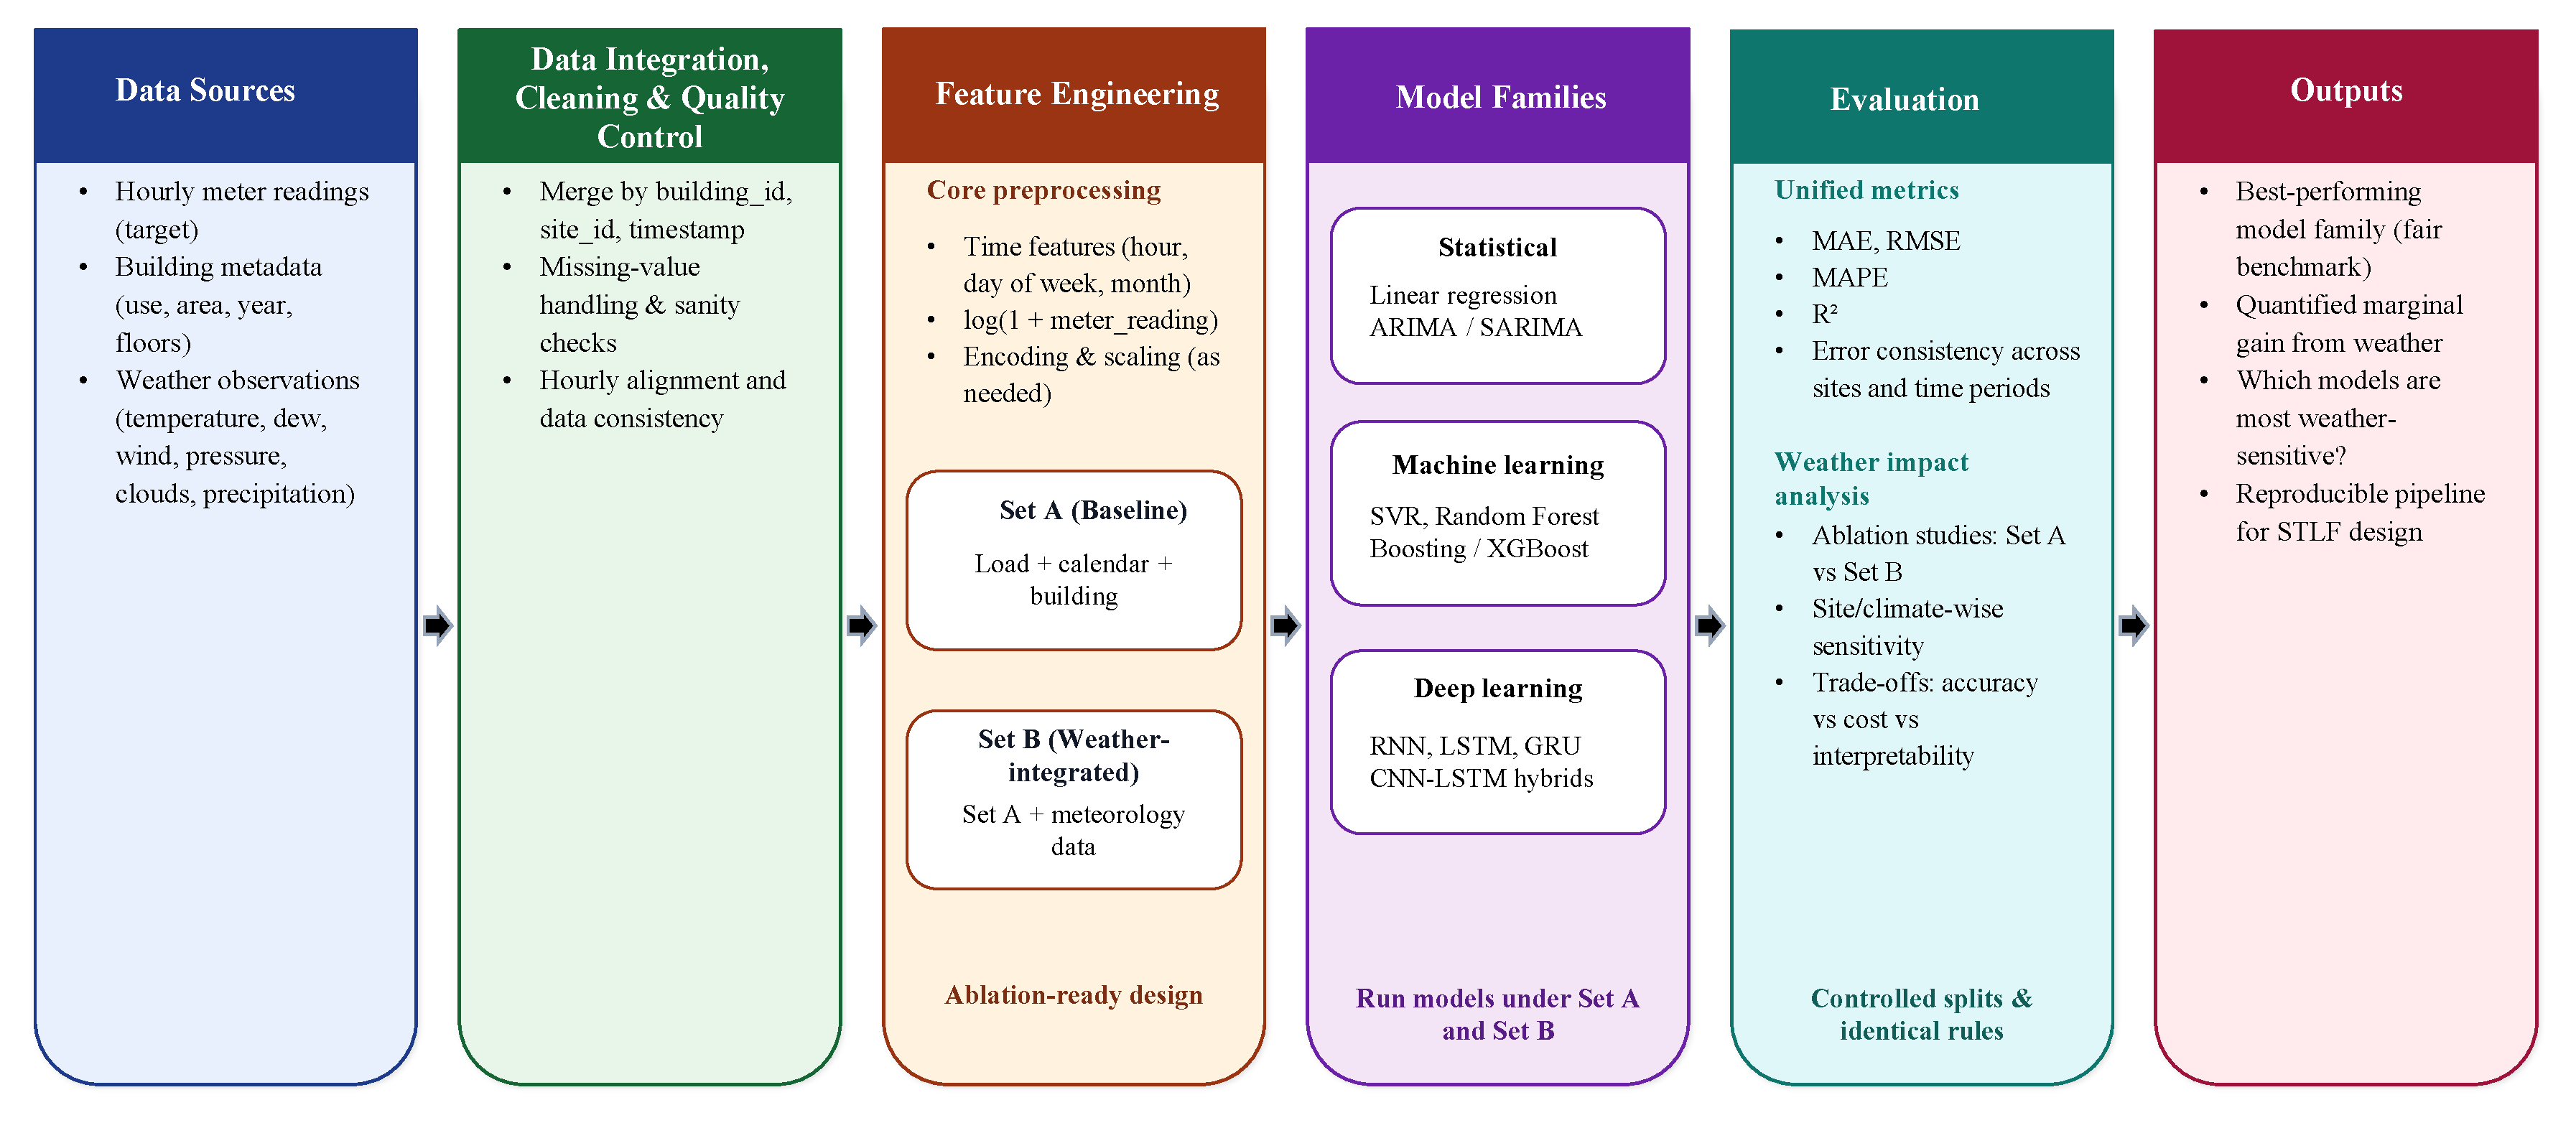
\includegraphics[width=\textwidth]{Framework.pdf}
    \caption{Proposed Unified Weather-Aware STLF Framework.}
    \label{fig:Framework}
\end{figure*}

After integration, the data move into the feature engineering stage. At this point, the raw inputs are transformed into model-ready predictors through steps such as extracting time-based variables, applying a logarithmic transformation to the target, and encoding or scaling variables where necessary. Two input sets are then created for comparison. The first is a baseline feature set built from load history, calendar information, and building characteristics. The second adds meteorological variables to that baseline so that the influence of weather can be tested directly.

These feature sets are then used across three groups of forecasting models: statistical methods, machine learning methods, and deep learning methods. By running all model families under both the baseline and weather-enhanced settings, the framework supports a fair and consistent comparison. Performance is then assessed using common error metrics and by examining how results vary across sites and time periods. Finally, the framework includes a weather-impact analysis to determine how much forecast accuracy improves when weather information is added, which model types are most sensitive to weather conditions, and what trade-offs exist among accuracy, cost, and interpretability. Overall, the framework is designed to produce a reproducible benchmark for short-term load forecasting while also making the role of weather in forecasting performance much clearer.

\subsection{Dataset Description}

This study utilizes the ASHRAE Great Energy Predictor III dataset, a large-scale real-world benchmark dataset for building-level energy forecasting. After integrating building metadata and weather information with the training dataset, the final merged dataset contains 20,216,100 observations and 16 variables.

The dataset spans from January 1, 2016 to December 31, 2016 at hourly resolution, covering 1,449 unique buildings distributed across 16 distinct sites. Each observation corresponds to a specific building, meter type, and timestamp.

The target variable is \texttt{meter\_reading}, representing energy consumption. Predictor variables include:

\begin{itemize}
    \item Building characteristics (primary use, square footage, year built, floor count)
    \item Temporal features (hour, day of week, month, year)
    \item Meteorological variables (air temperature, dew temperature, wind speed, sea level pressure, cloud coverage, precipitation depth)
\end{itemize}

The diversity of building types and climate conditions makes this dataset suitable for structured comparative forecasting and weather sensitivity analysis.

\subsection{Data Integration and Preprocessing}

The training dataset was merged with building metadata using \texttt{building\_id}, and subsequently merged with weather data using \texttt{site\_id} and \texttt{timestamp} as relational keys.

Exploratory analysis revealed significant missingness in certain structural and environmental variables:

\begin{itemize}
    \item floor\_count: 82.65\% missing
    \item year\_built: 59.99\% missing
    \item cloud\_coverage: 43.66\% missing
    \item precipitation depth (1hr): 18.54\% missing
\end{itemize}

Weather variables such as air temperature and dew temperature exhibited less than 0.5\% missing values.

Temporal features were extracted from timestamps, including hour-of-day and day-of-week indicators. Due to extreme right-skewness of the target variable (skewness = 104.81), logarithmic transformation was applied to stabilize variance and improve model suitability.


\subsection{Research Questions}

This study is guided by the following research questions:

\begin{enumerate}
    \item How do different forecasting paradigms (statistical, machine learning, and deep learning models) compare under a unified preprocessing and evaluation framework for short-term electricity load forecasting?

    \item To what extent does the integration of meteorological variables improve predictive performance?

    \item Which models demonstrate higher sensitivity to weather variables under varying climatic conditions?
\end{enumerate}

\subsection{Preliminary Exploratory Findings}

Exploratory analysis confirms strong temporal structure in electricity consumption. Average hourly load patterns reveal clear intra-day cyclic behavior, with peak demand observed in mid-afternoon hours. Weekly aggregation indicates elevated demand during mid-week relative to weekends.

Correlation analysis between meter readings and meteorological variables indicates weak linear correlation between raw load and air temperature (r = -0.004). However, nonlinear scatter patterns suggest potential non-linear relationships not captured by simple correlation coefficients.

Weather variables such as air temperature and dew temperature exhibit strong inter-correlation (r = 0.75), indicating multicollinearity considerations for model development.

These findings motivate a structured comparative modeling framework incorporating weather feature sensitivity analysis.



\bibliographystyle{IEEEtran}
\bibliography{References}

\end{document}
